\chapter{Implementation}
\label{chap:Impl}
\section{Programming APIs}

To implement applications, we can work directly with the SDK provided from each headset manufacturer, the advantage is that we can interact at a low level with the devices.\\ 
Another way is to use an SDK of a well-defined standard for example OpenVR from Valve or OpenXR from the Khronos group. This allows us to write applications for a target group of devices like room-scale supporting headsets without having to deal with different manufacturer SDKs (see Figure \ref{fig:openxr-overview}). On a side note: the X in OpenXR means that the specification is not only used for virtual reality (VR) applications but also for augmented reality (AR) and other technologies (XR) possibly proposed in the future.\\
Lastly, we can work with different engines which will provide with additional features. While classical desktop engines rely on downloading complete bundled packages for distributing the application, WebXR and WebVR allow us to distribute and run our application via the browser, similar to WebGL.

At the time of writing, the OpenXR and WebXR specification is still relatively new being in its first revision therefore it is not implemented by each headset manufacturer, browser and engine yet. However, these standards are meant to replace the old OpenVR and WebVR in the future.

\begin{figure}[h]
    \centering
    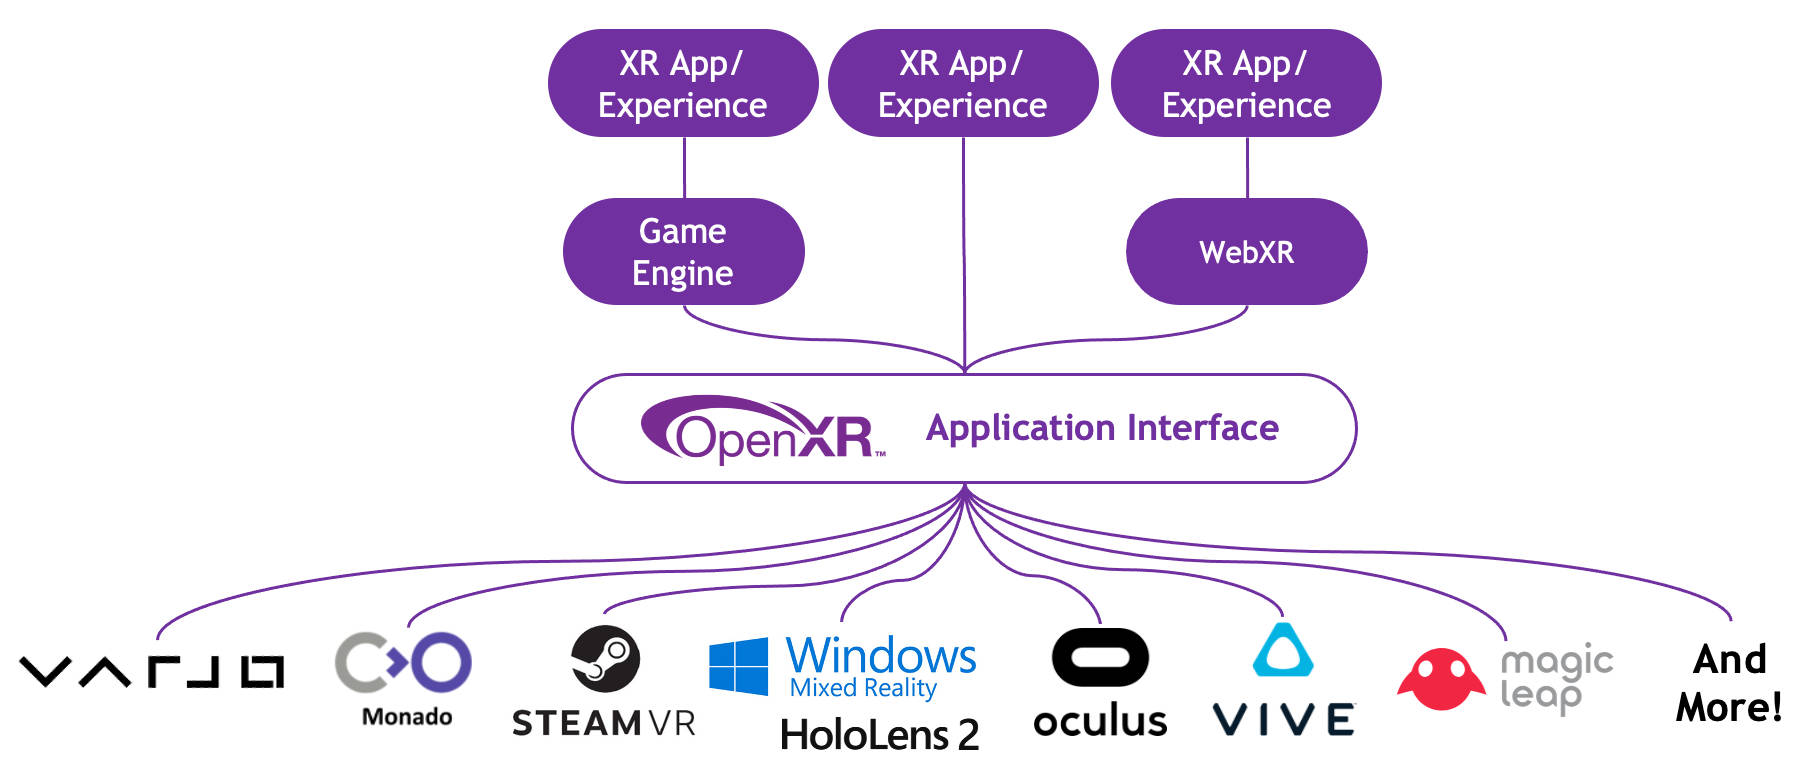
\includegraphics[width=\textwidth]{graphics/openXR-overview.jpg}
    \caption{Overview of the OpenXR API Stack \cite{khronosGroupOpenXR}}
    \label{fig:openxr-overview}
\end{figure}


\section{Preprocessing Scripts}

Flexible transforming any CSV Data to our own data format \\
generation of test data \\
coloring, filtering, ... parameter \\
File Format of final processed .JSON for the actual web-based visualization \\

\section{Position}
\subsection{D3-Forces}
List of used forces and its strength/importance, why is each force included
\subsection{Optimization}
Separate Forces per layer and calculating them successively.

\section{Rendering}
\subsection{Instanced nodes}
\subsection{Transparency}
\subsection{Visability}
Nodes (wireframe), Links ausblenden.

\section{VR Interactions}
\subsection{Camera Rig vs Camera}
camera rotation, correct position 
\subsection{Flyspeed}
\subsection{Button Mapping}
\subsection{Raycast(nur bei Bedarf da keine eigene Implementerung)}

\section{Scale}
\subsection{Scale of layer components}
Scale of nodes, link, label, ...
\subsection{Scaling interactions}

IDEE:\\
Vergleichsbild: links: 1x scale, rechts: 3x scale mit controller als referenz in jedem Bild\\
Vergleich zu room scale vs Table VR scale (paper)\\
subgraph kann als "Tisch" dargestellt werden, 
\\
Relevant Paper: \\
Axelsson\\
Dynamic Scene Graph: Enabling Scaling, Positioning, and Navigation in the Universe


\subsubsection{Manual scaling}
\subsubsection{Automated scaling}
